\documentclass{article}
% basics
\usepackage{amsfonts}
\usepackage{enumitem}
\usepackage{float}
\usepackage{graphicx}
\usepackage{hyperref} 
\usepackage[labelfont=bf]{caption}
\usepackage{algpseudocode}

\newtheorem{theorem}{Theorem}
\newtheorem{lemma}[theorem]{Lemma}
\newtheorem{corollary}{Corollary}[theorem]

% unique math expressions:  
\usepackage{amsmath}
\DeclareMathOperator*{\andloop}{\wedge}
\DeclareMathOperator*{\pr}{Pr}
\DeclareMathOperator*{\approach}{\longrightarrow}
\DeclareMathOperator*{\eq}{=}

% grey paper
\usepackage{xcolor}
% \pagecolor[rgb]{0.11,0.11,0.11}
% \color{white}

% embedded code sections
\usepackage{listings}
\definecolor{codegreen}{rgb}{0,0.6,0}
\definecolor{codegray}{rgb}{0.5,0.5,0.5}
\definecolor{codepurple}{rgb}{0.58,0,0.82}
\lstdefinestyle{mystyle}{
    commentstyle=\color{codegreen},
    keywordstyle=\color{magenta},
    numberstyle=\tiny\color{codegray},
    stringstyle=\color{codepurple},
    basicstyle=\ttfamily\footnotesize,
    breakatwhitespace=false,         
    breaklines=true,                 
    captionpos=b,                    
    keepspaces=true,                 
    numbers=left,                    
    numbersep=5pt,                  
    showspaces=false,                
    showstringspaces=false,
    showtabs=false,                  
    tabsize=2
}

\usepackage{tikz}
\usetikzlibrary{calc,arrows,positioning}

\newcommand{\lv}[0]{\overline{v}}
\newcommand{\lx}[0]{\overline{x}}

\lstset{style=mystyle}

\begin{document}
\tikzset{
    treenode/.style = {align=center},
    c/.style = {treenode,circle,draw=black,minimum width=1.5em,minimum height=1.5em,text centered,font=\footnotesize},
    r/.style = {treenode,rectangle,draw=black,minimum width=1.5em,minimum height=1.5em,text centered,font=\footnotesize},
    level 1/.style={sibling distance=60mm},
    level 2/.style={sibling distance=30mm},
    level 3/.style={sibling distance=15mm},
    level 4/.style={sibling distance=7mm}
}
\author{Yosef Goren}
\title{Software Verification Homework 4}
\maketitle

\section{BDD constructions}
%enumerate with letters:
\begin{enumerate}[label=\textbf{\alph*.}]
    \item 
        Denote the set of vertices: $V=\{\lx_i\mid i\in[n]\}$\\
        Let $E(\lv):=E_0(\lv)\wedge E_1(\lv)$.
        \[
            A'(\lv):=A(\lv)\wedge \left(\bigwedge_{i=0}^n(E(\lv,\lx_i)\Rightarrow B(\lx_i))\right)
        \]
        The idea is that $A(\lv)$ means the 'accepted' node has to be from $A$,
        and rest of the expression means that all of it's neighbors have to be in $B$.
        It is equivalent to satisfying the following formula:
        \[
            (\lv\in V)\wedge \left(\forall \lx\in V, E(\lx, \lv)\rightarrow B(\lx)\right)
        \]
    \item 
        \[
            V_{1,2}(\lv,\lv'):=
                \left(\bigvee_{i=0}^nE_1(\lv, \lx_i)\wedge E_0(\lx_i, \lv')\right)
                \vee
                \left(\bigvee_{i=0}^nE_0(\lv, \lx_i)\wedge E_1(\lx_i, \lv')\right)
        \]
        For the vertices $\lv,\lv'$ to have a 
        path of length 2 and weight 1 between them,
        there must either be a path of length 2 with weight
        1 were the edge connected to $\lv$ is 1 and the other edge is 0,
        or the other way around.\\
        The primary operator of the expression above describes this fact;
        to be more specific - the left side of the expression
        describes the case where there is a path of length 2 
        were the node connected to $\lv$ has weight 1, and so on.
    \item The algorithm works as follows:
    \begin{algorithmic}
        \State $T(v)\leftarrow\emptyset$
        \State $T'(v)\leftarrow A(v)$
        \State $l\leftarrow 0$ (*).
        \While{$T'(V)\neq T(v)$}
            \While{$T'(V)\neq T(v)$}
                \State $T(v)\leftarrow T'(v)$
                \State $T'(v)\leftarrow T'(v)\wedge\left(\bigvee_{i=0}^nE_0(v,v_i)\right)$
                \If{$B(v)\wedge T'(v)\neq\emptyset$}
                    \State \Return $l$
                \EndIf
            \EndWhile
            \State $T(v)\leftarrow T'(v)$
            \State $T'(v)\leftarrow T'(v)\wedge\left(\bigvee_{i=0}^nE_1(v,v_i)\right)$
            \State $l\leftarrow l+1$
            \If{$B(v)\wedge T'(v)\neq\emptyset$}
                \State \Return $l$
            \EndIf
        \EndWhile
        \State \Return $-1$
    \end{algorithmic}
    (*) $l$ represents the maximal minimum path from $A$ to any node in the working set $T$.\\

    The idea of the algorithm is to start with the set of states
    of $A$, then in each iteration expand our working set;
    if we can expand without increasing the weight of the newly formed paths -
    then we do that (expand only with edges of weight 0),
    if we cannot expand without increasing the weight - 
    we expand with edges of weight 1.\\
    After each such exapnsion we check if we have reached a state from $B$,
    and if so - we know we have a found the 'first' path into $B$ in terms of path weight -
    in other words - we have found a minimal path.

    Note that while there is a nested loop in this algorithm,
    it's total number of iterations is bounded by $n$ since
    in each iteration the length (*) of the maximal minimum path increases by once,
    and since the maximal length of any simple (and hence any minimal) path 
    is bounded by $n$ - the total number of iterations is bounded by $n$.
    
    (*) length in terms of in terms of distance, not weight.
\end{enumerate}
    
\section{BDD operations}
\begin{enumerate}[label=\textbf{\alph*.}]
\item
    \begin{enumerate}[label=\textbf{\arabic*.}]
    \item True. $D\subseteq D'$.\\
        Proof:\\
        Let $x\in D$. Denote the path of $x$ on $B$ with $a_1,a_2,...,a_n$.\\
        Since $x\in D$ then $B(x)=1$, meaning the path must end with $1$.
        If $\exists i\in[n]: a_i=u$.
        then on the evaluation of $x$ on $B'$,
        the path will be $a_1,a_2,...,a_{i-1},u,1$.
        Thus $B'(x)=1$ and so $x\in D'$ in this case.\\
        Otherwise, $x\notin D$. Thus the path $a_1,...,a_n$ is
        unchanged in $B'$ w.r. to $B$. Hence $B'(x)$ evaluates
        on the exact same path - which we know ends with $1$.
        Hence $B'(x)=1$ too, so $x\in D'$.\\
        Meaning in all cases $x\in D'$.\\
        So $D\subseteq D'$.
    \item False. %$D'\subsetneq D$.\\
        Counter example:\\
        Consider kripke structure $(S=\{0,1\},R=\{(s,s)\mid s\in S\},L=\{(s,\emptyset)\mid s\in S\})$.
        Consider $D=\{1\}$.\\
        Let $B$ be the BDD representing $D$:\\
        \begin{center}\begin{tikzpicture}[->,>=stealth',thick]
        \node[c]{$a_0$}
            child{ node[r] {0}}
            child{ node[r] {1}}
        ;\end{tikzpicture}\end{center}
        Now consider $u$ as $a_0$. This would mean $B'$ is: aa asdas
        \begin{center}\begin{tikzpicture}[->,>=stealth',thick]
        \node[c]{$a_0$}
            child{ node[r] {1}}
        ;\end{tikzpicture}\end{center}
        (Technically the $a_0$ would be reduced...).\\
        So now $B'(0)=1$ also, hence $D'=\{0,1\}\not\subseteq D$.
    \end{enumerate}
    \item
    \begin{enumerate}[label=\textbf{\arabic*.}]
        \begin{enumerate}[label=\textbf{\roman*.}]
            \item True. $R\subseteq R'$.\\
                For the same reason as before, if we have a BDD $B_i$
                representing set $S_i$ for $i\in\{0,1\}$ and
                were $B_1=cut(B_0)$ then regardless of the context $S_0\subseteq S_1$
                since we only increase the set of inputs that evaluate to $1$.
            \item False. $R'\not\subseteq R$.\\
                Consider a similar counterexample (as in a.2.):\\
                The structure:
                \[(S=\{0,1\},R=\{(s,s)\mid s\in S\},L=\{(s,\emptyset)\mid s\in S\})\]
                The BDD of $R(s_0,s_1)$ be $B$: (if $0$ go to left son)
                \begin{center}\begin{tikzpicture}[->,>=stealth',thick]
                \node[c]{$s_0$}
                    child{
                        node[c] {$s_1$}
                        child{ node[r] {1}}
                        child{ node[r] {0}}
                    }
                    child{
                        node[c] {$s_1$}
                        child{ node[r] {0}}
                        child{ node[r] {1}}
                    }
                ;\end{tikzpicture}\end{center}
                Let $u=s_0$ and $B'=cut(B,u)$: 
                \begin{center}\begin{tikzpicture}[->,>=stealth',thick]
                \node[r]{$s_0$}
                    child{
                        node[r] {1}
                    }
                ;\end{tikzpicture}\end{center}
                (After reduction just the leaf with 1 remains).\\
                Hence $R'=\{(0,0),(0,1),(1,0),(1,1)\}\not\subseteq R$
        \end{enumerate}
        \item No. This is since the change might create transisions 
            that don't even go into an existing vertex (state).\\
            For example, if we have $S:=\{0,1,2\}$ represented in binary as $S:=\{00,01,10\}$,
            and say we have some legal transition set $R\subseteq S\times S$, then we cat it's tree
            at the root node (like we did before), we will now have the set of all transitions on
            a pair of strings $(xy,zw)$ meaning:
            \[
                R'=\{(00,00),(00,01),(00,10),...,(11,10),(11,11)\}
            \]\[
                =\{(0,0),(0,1),...,(3,2),(3,3)\}    
            \]
            Among the rest, $R'$ contains $(3,2)$ for example -
            which makes no sense (and is not 'legal'); since $3\notin S$!
    \end{enumerate}
    \item
    \begin{enumerate}[label=\textbf{\arabic*.}]
        \item Yes. As described in \textbf{b.1.} - $R'\subseteq R$,
            meaning that all transisions that existed in $R$ also exist in $R'$.
            Moreover - this means that any path in $R$ is also a path in $R'$.\\
            Hence the set of paths considered to evaluate $M',s\models AGp$ (*)
            contains the set of paths considered to evaluate $M,s\models AGp$; (**)
            so if all paths in $(*)$ satisfy the condition, then all the paths in $(**)$
            also do; in other words - if $M',s\models AGp$ is satisfied, so is $M,s\models AGp$.
        \item No. Take for example the structure $M$:
        \begin{center}
            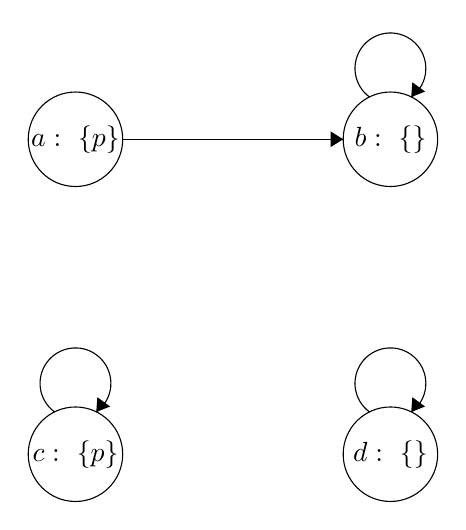
\begin{tikzpicture}[scale=0.2]
            \tikzstyle{every node}+=[inner sep=0pt]
            \draw [black] (3.2,-7) circle (3);
            \draw (3.2,-7) node {$a:\mbox{ }\{p\}$};
            \draw [black] (23.2,-7) circle (3);
            \draw (23.2,-7) node {$b:\mbox{ }\{\}$};
            \draw [black] (3.2,-27) circle (3);
            \draw (3.2,-27) node {$c:\mbox{ }\{p\}$};
            \draw [black] (23.2,-27) circle (3);
            \draw (23.2,-27) node {$d:\mbox{ }\{\}$};
            \draw [black] (6.2,-7) -- (20.2,-7);
            \fill [black] (20.2,-7) -- (19.4,-6.5) -- (19.4,-7.5);
            \draw [black] (21.877,-4.32) arc (234:-54:2.25);
            \fill [black] (24.52,-4.32) -- (25.4,-3.97) -- (24.59,-3.38);
            \draw [black] (1.877,-24.32) arc (234:-54:2.25);
            \fill [black] (4.52,-24.32) -- (5.4,-23.97) -- (4.59,-23.38);
            \draw [black] (21.877,-24.32) arc (234:-54:2.25);
            \fill [black] (24.52,-24.32) -- (25.4,-23.97) -- (24.59,-23.38);
            \end{tikzpicture}
        \end{center}
        Now cut the transitions set at the root node (which will cause all transitions to exist) like before to get the structure $M'$:
        \begin{center}
            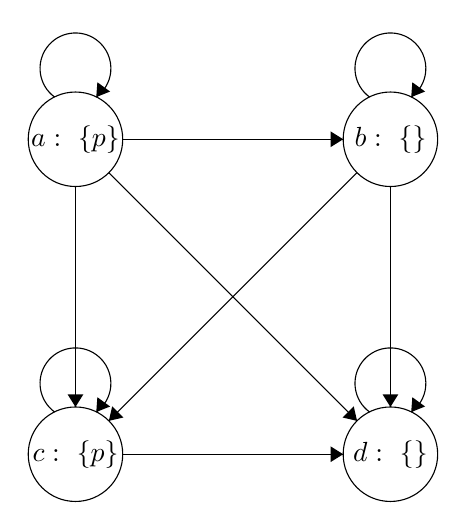
\begin{tikzpicture}[scale=0.2]
            \tikzstyle{every node}+=[inner sep=0pt]
            \draw [black] (3.2,-7) circle (3);
            \draw (3.2,-7) node {$a:\mbox{ }\{p\}$};
            \draw [black] (23.2,-7) circle (3);
            \draw (23.2,-7) node {$b:\mbox{ }\{\}$};
            \draw [black] (3.2,-27) circle (3);
            \draw (3.2,-27) node {$c:\mbox{ }\{p\}$};
            \draw [black] (23.2,-27) circle (3);
            \draw (23.2,-27) node {$d:\mbox{ }\{\}$};
            \draw [black] (6.2,-7) -- (20.2,-7);
            \fill [black] (20.2,-7) -- (19.4,-6.5) -- (19.4,-7.5);
            \draw [black] (3.2,-10) -- (3.2,-24);
            \fill [black] (3.2,-24) -- (3.7,-23.2) -- (2.7,-23.2);
            \draw [black] (5.32,-9.12) -- (21.08,-24.88);
            \fill [black] (21.08,-24.88) -- (20.87,-23.96) -- (20.16,-24.67);
            \draw [black] (21.08,-9.12) -- (5.32,-24.88);
            \fill [black] (5.32,-24.88) -- (6.24,-24.67) -- (5.53,-23.96);
            \draw [black] (23.2,-10) -- (23.2,-24);
            \fill [black] (23.2,-24) -- (23.7,-23.2) -- (22.7,-23.2);
            \draw [black] (6.2,-27) -- (20.2,-27);
            \fill [black] (20.2,-27) -- (19.4,-26.5) -- (19.4,-27.5);
            \draw [black] (1.877,-4.32) arc (234:-54:2.25);
            \fill [black] (4.52,-4.32) -- (5.4,-3.97) -- (4.59,-3.38);
            \draw [black] (21.877,-4.32) arc (234:-54:2.25);
            \fill [black] (24.52,-4.32) -- (25.4,-3.97) -- (24.59,-3.38);
            \draw [black] (1.877,-24.32) arc (234:-54:2.25);
            \fill [black] (4.52,-24.32) -- (5.4,-23.97) -- (4.59,-23.38);
            \draw [black] (21.877,-24.32) arc (234:-54:2.25);
            \fill [black] (24.52,-24.32) -- (25.4,-23.97) -- (24.59,-23.38);
            \end{tikzpicture}
        \end{center}
        If we define $s:=a$, then it is easy to see how $M',s\models EGp$ with
        the path $a\rightarrow c\rightarrow c\rightarrow c ...$.\\
        On the other hand, the only path that starts from $s$ ($a$) goes through $b$,
        hence it does not satisfy $Gp$.
    \end{enumerate}
\end{enumerate}


% \begin{tikzpicture}[->,>=stealth',thick] 
% \node[c] {a}
% node[c] {c}
%     child{ node[c] {d}
%         child{ node[r] {0}}
%         child{ node[r] {0}}
%     }
%     child{ node[c] {d}
%         child{ node[r] {0}}
%         child{ node[r] {1}}
%     }
% ;
% \end{tikzpicture}

\section{D\&D}
Solution for \textbf{a.+b.}\\
For the purpose of part \textbf{b.} we have assumed 
that the knight can only carry one princess at a time
and each dragon takes the princess away if reached.\\

In the solution we use the following notations:
\begin{enumerate}[label=\textbf{\arabic*.}]
    \item $\{v_i\mid i\in[n]\}$: the set of vertices ('squares').
    \item $V(v)$: a BDD representing the set of vertices.
    \item $E(v,v')$: a BDD representing the \textbf{REVERSE} set of edges (a transition from $v$ into $v'$).
    \item $S$: a BDD representing the set of starting vertecies.
    \item $F$: a BDD representing the set of final vertecies.
    \item $D$: a BDD representing the set of vertices with a dragon on them.
    \item $P$: a BDD representing the set of vertices with a princess on them.
    \item $N:=V\wedge\neg(S\vee F\vee D\vee P)$ (the set of 'normal' vertices).
    \item \[\Phi_U(v):=\bigvee_{i=1}^n(U(v)\wedge E(v,v_i))\]
        $\Phi_U$ is simply a 'macro' for ease of readability.\\
        Given a set $U$, $\Phi_U$ is the set of vertecies that are directly connected to a vertex in $U$.\\
        The evaluation $\Phi_U(v)$ is $1$ iff there is a vertex in $U$ that is connected to $v$.
\end{enumerate}

We present a single algorithm that can handle multiple dragons.\\
The structure of the algorithm is that we hold
multiple sets that are represented as BDDs, and we manipulate
these sets in each iteration s.t. when the algorithm ends,
one of them will contain the set of all valid paths.\\

In our algorithm we look for reverse paths, meaning paths from
a final state to a starting state - on a graph with reversed edges.\\

The main idea of the algorithm is that we will start with the
set of finishing squares,
and in each iteration 'expand' to all neighboring squares,
but if we encounter a dragon we will have to move
each node that was reached through a dragon into a new
set of 'debt' paths (more accurately - squares that were reached from an final square thorugh
a dragon square). Now if we step from a square with debt into
a starting square, we know the path is not valid, but if
we step from a square with no debt into a starting square,
then we know we have a path that started from a final square
and ended in a starting square were each dragon we have passed through
has be 'paid' for with a princess.\\
If we encounter a princess from the debt set - we can
move into the non-debt set,
if we encounter a princess from the non-debt set - 
we have 'no use' for her since all dragons
in the rest of the path have already been paid for (we have no debt!),
hence we stay in the non-debt set.\\

These transitions between the sets are described with the following atomata:\\

\begin{center}
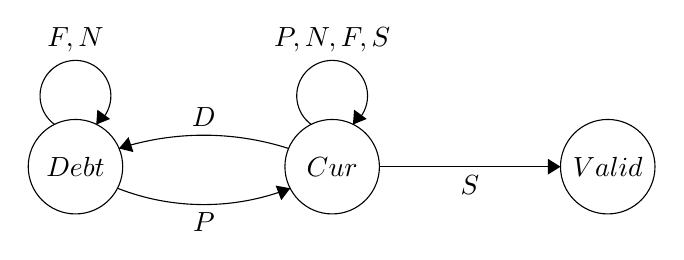
\begin{tikzpicture}[scale=0.2]
\tikzstyle{every node}+=[inner sep=0pt]
    \draw [black] (19.5,-9.1) circle (3);
    \draw (19.5,-9.1) node {$Cur$};
    \draw [black] (3.2,-9.1) circle (3);
    \draw (3.2,-9.1) node {$Debt$};
    \draw [black] (37,-9.1) circle (3);
    \draw (37,-9.1) node {$Valid$};
    \draw [black] (22.5,-9.1) -- (34,-9.1);
    \fill [black] (34,-9.1) -- (33.2,-8.6) -- (33.2,-9.6);
    \draw (28.25,-9.6) node [below] {$S$};
    \draw [black] (5.964,-7.944) arc (107.81821:72.18179:17.601);
    \fill [black] (5.96,-7.94) -- (6.88,-8.17) -- (6.57,-7.22);
    \draw (11.35,-6.6) node [above] {$D$};
    \draw [black] (1.877,-6.42) arc (234:-54:2.25);
    \draw (3.2,-1.85) node [above] {$F,N$};
    \fill [black] (4.52,-6.42) -- (5.4,-6.07) -- (4.59,-5.48);
    \draw [black] (18.177,-6.42) arc (234:-54:2.25);
    \draw (19.5,-1.85) node [above] {$P,N,F,S$};
    \fill [black] (20.82,-6.42) -- (21.7,-6.07) -- (20.89,-5.48);
    \draw [black] (16.836,-10.468) arc (-68.55273:-111.44727:15.003);
    \fill [black] (16.84,-10.47) -- (15.91,-10.3) -- (16.27,-11.23);
    \draw (11.35,-12.01) node [below] {$P$};
\end{tikzpicture}
\end{center}


The algorithm :
\begin{algorithmic}
    \State $Cur\leftarrow F, Debt\leftarrow\emptyset, Valid\leftarrow\emptyset$
    \For{$\_\in[n]$}
        \State Do the following 3 assigments atomically (*):
        \State $
            Cur\leftarrow
                \left(\Phi_{Cur}\wedge(P\vee N\vee F\vee S)\right)
                \vee
                \left(\Phi_{Debt}\wedge P\right)
        $
        \State $
            Debt\leftarrow
                \left(\Phi_{Cur}\wedge D\right)
                \vee
                \left(\Phi_{Debt}\wedge (F\vee N)\right)
        $
        \State $
            Valid\leftarrow
                \left(\Phi_{Cur}\wedge S\right)
        $
    \EndFor
    \State \Return $Valid$
\end{algorithmic}
(*) making a set of assignments atomically
means that all rvalues are evaluated before any
lvalues are assigned.\\


\end{document}